\documentclass[11pt]{article}
\usepackage[preprint]{acl}
\usepackage{times}
\usepackage{latexsym}
\usepackage[T1]{fontenc}
\usepackage[utf8]{inputenc}
\usepackage{microtype}
\usepackage{inconsolata}
\usepackage{graphicx}
\usepackage{booktabs}
\usepackage{amsmath,amssymb}
\title{Parallel Retrieval and Bounded Evaluation for Conversational Customer Service}
\author{HKUST NLP Project Team}
\begin{document}
\maketitle
\begin{abstract}
Customer-service questions depend on dialogue history and conditions distributed across policy documents. We integrate query planning, alternative retrieval paths, cited generation, and bounded evaluator-driven revision. The native fine-tuned path uses Dense rankings directly, without fusion or reranking; hybrid retrieval remains a comparator. Adapted Dense reaches 78.25 Hit@10 on a historical dummy-file development cohort, without establishing final-test superiority. Separately, saved MiniLM hybrid-pipeline results on 1,000 MultiDoc2Dial validation requests obtain token F1 of 20.80 and evidence Recall@5 of 68.13. On 20 synthetic cross-domain requests using that earlier backend, domain routing raises initial document recall from 60 to 75 percent. Independent domain generation costs more without a final coverage advantage. Evaluation adds one accepted question per arm but often replaces useful drafts with handoff messages. Conditional errors and unstable automatic grading motivate calibrated evaluation and stopping.
\end{abstract}
\section{Introduction}
An online customer-service assistant must recover what a user means, find the relevant policy, and preserve its qualifications when answering. A follow-up such as \emph{What should I bring?} is incomplete without the previous exchange. A compound request can also involve several services, such as replacing a driver's license while updating benefit-payment details. Retrieving a plausible paragraph is therefore only one part of the task: the answer must cover each requested item without transferring a condition from one policy statement to another.

Retrieval-augmented generation (RAG; \citealt{lewis2020rag}) provides external evidence, but a fixed retrieve-and-generate pass can fail through an unresolved query, missing evidence, or an unsupported interpretation of retrieved text. These failures need different responses. Missing user information calls for clarification; missing policy evidence calls for retrieval; an incomplete answer supported by existing evidence calls for revision. Repeating all stages indiscriminately adds cost and may reproduce the same error.

We investigate a modular system with dialogue planning, configurable retrieval, evidence-conditioned generation, and an evaluator--optimizer controller. Retrieval evolved from parallel hybrid search with optional reranking to an alternative adapted Dense path without either fusion or reranking. Agents are logical roles with structured interfaces; the language-model roles share DeepSeek Flash. The controller distinguishes evidence adequacy from answer completeness and selects bounded corrective actions.

Our investigation asks three downstream questions. Does routing a compound request to separate document domains improve evidence coverage? Does generating independent domain answers help beyond pooling the same evidence? Does evaluation-driven revision increase useful answer delivery at an acceptable cost? A complementary retrieval study examines segmentation, hybrid retrieval, reranking, and encoder adaptation.

Our contributions are a runnable integration with citations and resource controls, a native retrieval study of segmentation and adaptation, a 1,000-request single-pass development evaluation, and a paired 20-request study of routing and answer composition. The small study supports domain routing more strongly than additional generation stages. Evaluator approval and citation validity remain insufficient evidence of factual correctness; we report negative findings and protocol limitations alongside gains.

\section{Related Work}
\paragraph{Document-grounded dialogue and retrieval.}
MultiDoc2Dial \citep{feng2021multidoc2dial} studies goal-oriented dialogue grounded in multiple documents. Its service domains make contextual interpretation and policy qualifications central to answering. RAG \citep{lewis2020rag} combines retrieved evidence with generation. BM25 \citep{robertson2009bm25} provides lexical matching, while reciprocal rank fusion \citep{cormack2009rrf} combines rankings without requiring comparable raw scores. We investigate these established components as complementary evidence sources.

\paragraph{Conversational planning and iterative retrieval.}
CONQRR \citep{wu2022conqrr} learns to rewrite conversational questions for retrieval. Our planner instead uses prompted structured generation and does not train a rewriting policy. IRCoT \citep{trivedi2023ircot} interleaves retrieval with multi-step reasoning. Our loop acts on evidence and answer diagnoses; it does not reproduce IRCoT's reasoning procedure or its published evaluation. The cross-domain cases in our study are mostly parallel compound requests, so they should not be treated as a multi-hop benchmark.

\paragraph{Feedback and model-based evaluation.}
Self-Refine \citep{madaan2023selfrefine} iteratively improves outputs using model feedback, and Self-RAG \citep{asai2024selfrag} incorporates learned retrieval and reflection behavior. We use an external prompted evaluator and a deterministic action router, without training reflection tokens. Model judges can make evaluation scalable but exhibit biases and reasoning limitations \citep{zheng2023judging}. We therefore distinguish online policy decisions, automatic required-point grading, and reference-based metrics, and inspect cases where these signals disagree.

\section{System Methodology}
\label{sec:method}
\begin{figure*}[t]
\centering
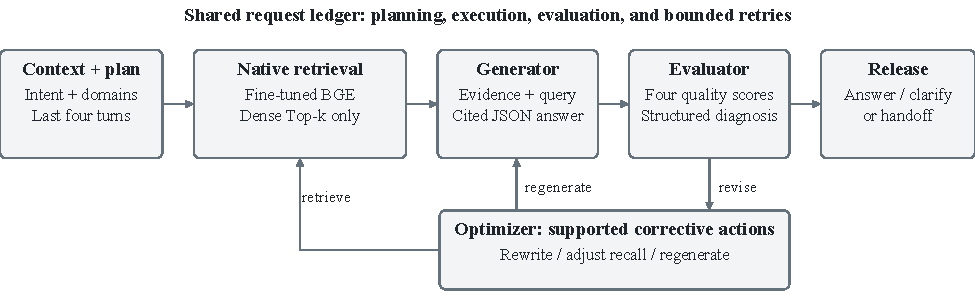
\includegraphics[width=\textwidth]{figures/architecture.pdf}
\caption{The selectable native fine-tuned configuration. Dense ranks are used directly without BM25, RRF, or Cross-Encoder reranking. Corrections are restricted to supported actions. Historical shared-model runs use the separate hybrid path; cross-domain continuation follows the branch-level protocol in Section~\ref{sec:setup}.}
\label{fig:architecture}
\end{figure*}

\subsection{Dialogue Planning}
The planner receives the current message and visible preceding turns. It returns a standalone query, intent, domain label, and optional subquestions. The domain is one of DMV, SSA, StudentAid, VA, or unknown. Unknown predictions may fall back to lexical cues in visible dialogue. The shared-model configuration allows at most three initial subquestions, normalizes whitespace, and removes duplicates. Gold domains, future turns, reference answers, and grounding labels remain outside online inputs.

The shared-model hybrid experiments use the standalone rewrite. For native fine-tuned retrieval, the initial query instead joins the last four visible user/agent turns with role labels and clears subqueries, matching retriever training. Domain prediction is advisory: global search is used unless a routing experiment explicitly applies predicted-domain filters. Gold metadata is not supplied to the planner.

% Integrated from retrievalreport_en.docx. Results are in 05_retrieval_existing.tex.
\subsection{Fine-Tuned and Hybrid Retrieval}
\label{sec:retrieval-method}
Two alternative paths share an evidence contract with stable document/passage IDs, source spans, and provenance. The current native fine-tuned preset selects struct passages and BGE checkpoint-2000, returning Dense cosine Top-10 directly. It disables BM25, RRF, Cross-Encoder reranking, subqueries, and additional semantic/per-document filtering. The retained hybrid path searches dense and lexical indexes in parallel, then fuses and optionally reranks candidates. These are alternatives, not consecutive stages of the fine-tuned path.

\paragraph{Structure-aware passages.}
Native index text joins the document title, ancestor titles, section title, and body. \emph{Section} groups spans by section ID and preserves standalone headings. \emph{Struct} merges adjacent spans sharing a section ID or stripped title, retaining a title path and coherent body. This keeps related policy sentences and conditions together, gives dense encoding a clearer subject, and lets BM25 match related terms within one passage. Fewer heading-only fragments compete for the final evidence slots. These are plausible mechanisms, rather than separately isolated effects.

\paragraph{Hybrid comparator and fusion.}
BGE-base-en-v1.5 uses 768-dimensional normalized CLS embeddings, a 512-token limit, its retrieval query prefix, and FAISS exact inner-product search. BM25 indexes the same passage text and removes user/agent query labels. Dense matching captures semantic similarity, while BM25 preserves exact service terms and form numbers. For the native hybrid study, Dense Top-100 and BM25 Top-50 are deduplicated and combined as
\begin{equation}
 \mathrm{RRF}(p)=\sum_{r:p\in L_r}
 \frac{1}{30+\mathrm{rank}_{L_r}(p)},
\end{equation}
where $L_r$ is a branch's ranked list. Fusion retains 50 candidates without comparing the branches' raw score scales.

\paragraph{Optional hybrid reranking.}
In the hybrid comparator, the MiniLM-L6-v2 MS MARCO Cross-Encoder jointly scores query--passage pairs. Its query places the current user question before earlier user questions. Short confirmations such as \emph{yes} keep RRF order because their meaning depends on the preceding agent turn. Pairwise inference adds query cost as candidate count and traffic grow. The fine-tuned path neither loads nor calls this model.

\paragraph{Dense adaptation.}
We also investigate replacing query-time reranking with an adapted Dense retriever. Training uses 20,607 deduplicated struct inputs and all 109.5M BGE parameters: AdamW, learning rate $2\!\times\!10^{-5}$, weight decay .01, batch size 8, 2,000 steps, gradient clipping at 1.0, warmup/decay, and seed 20261108. A scale-20 multi-positive contrastive loss rewards any labeled positive and masks unlabeled same-document negatives. Checkpoint 2000 is selected on dev160 (Hit@10 78.75, versus 77.50 at step 1000); document vectors are rebuilt for it. Adapted Dense directly ranks passages without BM25, RRF, or a Cross-Encoder. Section~\ref{sec:retrieval-study} compares the four native configurations.

\subsection{Cited Response Generation}
The generator receives the original request, standalone query, visible history, and retrieved evidence. The prompt exposes local aliases such as E1 and E2 and requests a JSON answer, citation list, and status. Aliases are mapped back to stable source IDs. An answered response must cite at least one supplied passage; an insufficient-evidence response must have no citations. Unknown citations and inconsistent recognized inline markers are rejected. One additional format-correction call is allowed using the same evidence and budget. These checks validate output structure and citation membership, rather than entailment.

\subsection{Evaluation and Action Selection}
The evaluator scores relevance, answer sufficiency, groundedness, and dialogue consistency on a zero-to-one scale. The respective thresholds are 0.7, 0.7, 0.8, and 0.8. A separate evidence-sufficiency field asks whether the current context could support a complete revision. This distinction prevents an answer omission from automatically being diagnosed as a retrieval failure.

Feedback specifies missing information, failure categories, suggested queries, and a proposed decision. Structured diagnoses take priority: misunderstanding suggests query rewriting, retrieval coverage suggests recall adjustment, ranking suggests reranking where supported, and answer defects suggest regeneration. The native fine-tuned path exposes no reranking capability; unsupported actions cannot silently enable a Cross-Encoder. Explicitly insufficient evidence redirects regeneration toward retrieval. Negative diagnoses, low scores, invalid citations, or non-answer status block approval. Missing user information may trigger clarification.

\subsection{Budgets and Stopping}
The application creates one ledger before planning and retains it throughout initial retrieval, generation, evaluation, and optimization. The real-model configuration allows 30,000 total tokens, 180 seconds, and two optimization retries, with a maximum of 1,024 output tokens per call. Before a call, the ledger reserves a conservative allowance; afterward it charges reported usage, including usage from rejected malformed responses. Unknown usage remains unavailable rather than becoming zero.

The controller stops on approval, clarification, escalation, a resource limit, unsupported actions, ineffective changes, or repeated unchanged state. Reusing adequate evidence for revision avoids unnecessary recall. An unchanged retrieval context normally stops the loop unless the diagnosis justifies answer revision. The retry bound counts optimization actions, not all model calls: format correction and separate evaluation calls also consume resources. Escalation prepares the dialogue, evidence, feedback, and attempted actions for handoff; the implementation does not deliver that package to a live human-service platform.

\section{Experimental Setup}
\label{sec:setup}
\subsection{Data and Evaluation Cohorts}
We use MultiDoc2Dial's 488 documents across DMV, SSA, StudentAid, and VA. The shared preprocessing produces 3,798 character-window passages with a maximum window size of 800 characters and 120-character overlap. Consecutive user turns and following agent turns form request--response examples. A seeded dialogue-level split of the official training data yields 20,558 training and 2,248 development requests; official validation contains 4,427 requests. Earlier turns alone form online history.

Official grounding offsets define evidence groups: overlapping windows that cover the same fragment are alternatives, while fragments needed for a long span are jointly required. The development mini set is drawn from the training-derived development split.

We keep three evaluation cohorts separate. First, the retrieval component compares section/struct corpora and encoder variants. The distributed v1.0 test file is explicitly documented as a dummy file; its 400-query historical comparison is reported only as development evidence. Second, a seed-42 sample of 1,000 official validation requests measures the single-pass downstream pipeline. Third, 20 AI-assisted synthetic cross-domain requests compare three orchestration designs. Their 84 required points and source annotations await independent human review; 19 requests are parallel compound questions. Validation has been used for development, so it is not an untouched final test set. HotpotQA was considered but has not been adapted or evaluated.

\subsection{Models and Controlled Comparisons}
The retrieval study uses BGE-base-en-v1.5 with 768-dimensional embeddings and native FAISS indexes. The current native preset selects adapted Dense without reranking. The saved downstream studies instead use frozen 384-dimensional all-MiniLM-L6-v2 embeddings, the character-window corpus, a MiniLM Cross-Encoder, and \texttt{deepseek-flash} at temperature zero. Their results are not reattributed to fine-tuned BGE; no matched large-scale downstream rerun with it is available.

The 1,000-request pipeline includes planning, hybrid retrieval, RRF, reranking, and generation, with evaluation and optimization disabled. It is a single-pass hybrid comparator, not a Dense-only Single-RAG baseline.

For the 20-request study, A retrieves globally and generates jointly; B retrieves separately within predicted domains and pools evidence for one answer; C generates domain-specific answers and then synthesizes them against the original evidence. One multilabel plan is shared across arms, and initial B/C evidence IDs and order match for every request. The final context budget is six passages. With two domains, each receives three passages and half the nominal Dense/BM25 candidate quota. A uses Dense/BM25 Top-50, RRF candidate depth 30; B/C use Top-25 and depth 15 per domain.

The later batch reuses saved initial answers. A continues to search globally, B retains domain-filtered branches, and C optimizes domain answers separately before final synthesis. C's final revision cannot fetch new cross-domain evidence. Each historical branch workflow has its own 30,000-token/180-second ledger and two-retry limit, seeded with initial generation tokens and elapsed generation time. These ledgers exclude shared planning and original retrieval, and do not impose a shared end-to-end budget on the whole C arm.

\subsection{Metrics and Accounting}
For official requests, we report reference token F1, exact match, evidence-group Recall@$k$, citation validity, latency, and tokens. Recall uses the post-fusion/post-reranking candidate list, before truncation to the five-passage generation context. Unanswered reference-bearing cases score zero on F1/EM. For synthetic cases, required-point coverage is
\begin{equation}
 \mathrm{Cov}=\frac{1}{N}\sum_{i=1}^{N}
 \mathbf{1}[s_i=\mathrm{answered}]
 \frac{|\widehat{P}_i\cap P_i|}{|P_i|},
\end{equation}
where the same model family grades which annotated points appear in the answer. Non-answered cases score zero. We separately report online acceptance and annotated source-document recall in the final context. Neither metric is factual accuracy.

Per-arm pipeline tokens include generation and online evaluation, including C's subworkflows, but exclude the shared planner (321.4 tokens/request) and offline grading. Added workflow time excludes the original execution. The 1,000-request cost summary retains the last attempt per sample and omits outer recovery retries. We therefore avoid comparing its latency directly with the continuation times. Exploratory paired intervals resample the 20 question indices 50,000 times with seed 42; they do not measure annotation or judge uncertainty.

\section{Results}
\label{sec:results}
% Results integrated from retrievalreport_en.docx. The original DOCX is unchanged.
% The 400-query cohort is corrected to development because its source is dummy test.
\subsection{Conversational Retrieval and Reranking}
\label{sec:retrieval-study}
We first evaluate the native retrieval methods in Section~\ref{sec:retrieval-method}, before studying downstream orchestration. Table~\ref{tab:segmentation} summarizes corpus sizes and encoder input lengths, including special tokens.

\begin{table}[t]
\centering\small
\setlength{\tabcolsep}{3.5pt}
\begin{tabular}{lrrrr}
\toprule
Corpus & Passages & Median & P95 & $>512$\\
\midrule
Section & 13,421 & 47 & 129.0 & 0.06\%\\
Struct & 4,110 & 116 & 390.5 & 2.70\%\\
\bottomrule
\end{tabular}
\caption{Native corpus sizes and input token lengths.}
\label{tab:segmentation}
\end{table}

A matched comparison uses the same 160 validation queries, visible four-turn history, BGE model, and global search. Original span IDs map next-agent grounding into each corpus. Struct improves Dense and RRF Hit@10 by approximately 20.6 and 22.5 points (Table~\ref{tab:segment-results}), while storing 69.4\% fewer passage vectors. However, grouping and title formatting change together; longer passages also consume more context and can mix conditions. Equal Top-10 counts are not equal token budgets, and 2.70\% of struct inputs exceed 512 tokens. These results support the combined struct design here without isolating its mechanisms.

\begin{table}[t]
\centering\small
\setlength{\tabcolsep}{4pt}
\begin{tabular}{lrrr}
\toprule
Corpus and method & Hit@10 & Recall@10 & MRR@10\\
\midrule
Section Dense & 41.88 & 41.88 & .1957\\
Section RRF & 46.88 & 46.88 & .2109\\
Struct Dense & 62.50 & 62.50 & .3369\\
Struct RRF & 69.38 & 69.38 & .4267\\
\bottomrule
\end{tabular}
\caption{Matched segmentation comparison ($n=160$). Hit, passage recall, and span recall coincide on this cohort; percentages are reported for Hit and recall.}
\label{tab:segment-results}
\end{table}

\begin{table}[t]
\centering\small
\setlength{\tabcolsep}{3.5pt}
\begin{tabular}{lrrrrr}
\toprule
Arm & H/R@10 & MRR & nDCG & H@50 & ms\\
\midrule
R1 & 59.75 & .3505 & .4100 & 82.75 & 8.5\\
R2 & 78.25 & .5286 & .5904 & 93.25 & 10.4\\
R3 & 66.25 & .3832 & .4496 & 87.00 & 45.4\\
R4 & 74.50 & .5307 & .5834 & 87.00 & 100.8\\
\bottomrule
\end{tabular}
\caption{Balanced 400-query dummy-file development comparison. R1: untuned Dense; R2: adapted Dense; R3: hybrid RRF; R4: R3 + Cross-Encoder. Hit/Recall (H/R) coincide because each query has one gold passage. MRR and nDCG use cutoff 10; H@50 is candidate hit rate. Hit/Recall are percentages; latency is mean CUDA query time.}
\label{tab:retrieval-adaptation}
\end{table}

Adapted Dense has the highest observed Hit@10: 18.50 points above untuned Dense and 3.75 above hybrid reranking (Table~\ref{tab:retrieval-adaptation}). Reranking has slightly higher MRR (.5307 versus .5286), whereas adaptation has higher nDCG and candidate coverage. Adaptation's recorded query latency is about 89.7\% lower than reranking's. Its 3.75-point Hit advantage has a dialogue-cluster bootstrap interval of $[-0.72,8.17]$ points; a reliable superiority claim is unwarranted even before considering dummy-file provenance and a single seed.
R4 reranks untuned hybrid retrieval, not adapted Dense. No adapted-Dense-plus-Cross-Encoder arm was evaluated, so omitting reranking is a configuration choice, not proof that it could never help an adapted encoder.

\subsection{Official Validation Single Pass}
\label{sec:official-results}
\begin{table}[t]
\centering\small
\begin{tabular}{lr}
\toprule
Metric ($n=1,000$) & Value\\
\midrule
Answered / insufficient / error & 973 / 25 / 2\\
Response token F1 / EM & 20.80 / 0.00\\
Evidence Recall@1 / @5 / @10 & 40.00 / 68.13 / 77.03\\
Citation ID validity & 100.00\\
Citation gold precision & 32.22\\
Mean / P95 latency (seconds) & 4.73 / 6.05\\
Mean model calls / tokens & 2.02 / 2,127\\
\bottomrule
\end{tabular}
\caption{Single-pass validation development results. Quality metrics are percentages. Costs describe each sample's final attempt; citation membership does not establish factual support.}
\label{tab:official}
\end{table}

Table~\ref{tab:official} establishes a functioning reference-based comparator, not an improvement from optimization. Evidence Recall@10 exceeds Recall@5 by 8.90 points, suggesting that some annotated evidence remains below the five-passage final context. Increasing context is therefore a plausible coverage intervention, but its effect on answer quality and token use requires a matched experiment.

The gap between valid citations and gold precision shows that structural citation checks solve only one problem. A supplied passage can fall outside the annotated gold alternative-passage set; this mismatch does not itself establish unsupported claims. Token F1 and EM are sensitive to wording and answer length, so they cannot independently diagnose factual errors. The two retained errors violate the output contract by attaching citations to insufficient-evidence answers after format correction. No full-loop run on the same 1,000 requests is available.

\subsection{Routing and Independent Generation}
\begin{table}[t]
\centering\small
\setlength{\tabcolsep}{4pt}
\begin{tabular}{lrrr}
\toprule
Metric ($n=20$) & A & B & C\\
\midrule
\multicolumn{4}{l}{Initial single pass}\\
Source-document recall & 60.00 & 75.00 & 75.00\\
Required-point coverage & 48.08 & 56.75 & 60.67\\
All points covered (count) & 1 & 2 & 3\\
Mean generation tokens & 1,732 & 1,759 & 4,528\\
\midrule
\multicolumn{4}{l}{After evaluation and bounded optimization}\\
Source-document recall & 55.00 & 75.00 & 67.50\\
Delivered point coverage & 12.50 & 45.00 & 43.25\\
Answered (count) & 3 & 14 & 12\\
All points covered (count) & 1 & 2 & 3\\
Mean pipeline tokens & 7,313 & 6,866 & 14,756\\
Mean pipeline calls & 3.45 & 3.20 & 9.05\\
\bottomrule
\end{tabular}
\caption{Cross-domain development study. Coverage and recall are percentages; non-answered outputs receive zero delivered point coverage. A: global retrieval; B: routed retrieval and pooled generation; C: routed retrieval, separate answers, and synthesis.}
\label{tab:crossdomain}
\end{table}

Under the same initial context limit, routed retrieval raises annotated document recall by 15 points (Table~\ref{tab:crossdomain}). B improves initial point coverage over A by 8.67 points, but its exploratory paired interval spans zero ($[-0.33,17.83]$). Many questions directly name their agencies, and predicted domain sets match annotations for all 20 requests; this does not establish routing accuracy for implicit or unseen requests.

Because initial B/C evidence matches, their comparison isolates answer composition more closely. C initially gains 3.92 coverage points, concentrated in three questions, while consuming 2.58 times B's generation tokens. After evaluation and optimization, C's coverage is 1.75 points below B ($[-9.00,3.75]$), and its pipeline token use is 2.15 times higher. The added computation has no aggregate coverage advantage on this cohort.

\subsection{What the Loop Changes}
Final online acceptance increases from 10 to 15\% for A, 65 to 70\% for B, and 55 to 60\% for C's final synthesis. Each arm adds only one accepted question, case 010. C's domain-level workflows separately improve from 17/40 to 22/40 accepted outputs and include one internal contract error. Domain-level counts should not be added to final-answer acceptance.

The larger final B--A coverage difference of 32.50 points ($[17.25,48.33]$) partly reflects abstention: A returns an escalated status on 17 questions. Fourteen A workflows stop after unchanged context and three reach the retry limit. Thirty initially credited points in those questions disappear from final delivery when generic handoff messages replace drafts. Lower delivered coverage therefore does not demonstrate that every revised draft became worse, while higher acceptance does not prove factual correctness.

\section{Discussion and Error Analysis}
\label{sec:discussion}
\begin{figure}[t]
\centering
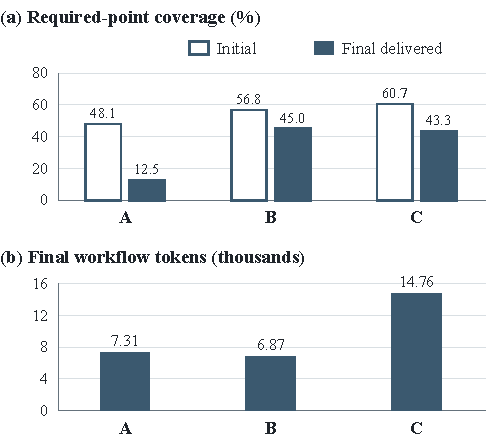
\includegraphics[width=\linewidth]{figures/coverage_cost.pdf}
\caption{The 20-case coverage--cost tradeoff. Top: initial and final delivered point coverage. Bottom: total model tokens per workflow, including evaluation but excluding shared planning and offline grading. Stages use different accounting scopes, so token bars show only the final workflow.}
\label{fig:tradeoff}
\end{figure}

\subsection{Retrieval Quality and Maintenance Cost}
Struct offers coherent evidence with fewer vectors, at the cost of coarser matches, more tokens per passage, and truncation risk. Adapted Dense shifts work offline: changing encoder weights requires training and re-encoding the corpus. Frozen retrievers with an off-the-shelf reranker avoid task-specific training but add candidate-pair scoring on every query. In principle, either a frozen adapted or untuned encoder can encode new documents without retraining; an incremental-update workflow was not evaluated. Total training, rebuilding, and maintenance costs were not systematically compared, so query latency is not a deployment-cost comparison. These BGE results do not establish downstream gains for the separate MiniLM backend.

\subsection{Routing Helps Before More Agents Help}
The matched initial B/C retrieval results suggest that the main gain comes from allocating context across domains, rather than from generating more intermediate answers. Independent generation can help locally: in case 017, the synthesized answer includes the bank-account detail missing from the pooled answer. This is useful evidence that decomposition can recover an omitted requirement, but three improved initial cases and higher aggregate cost do not justify unconditional decomposition. A sensible next experiment would trigger independent generation only after identifying uncovered subrequests.

\subsection{Approval Can Miss a Conditional Error}
Case 018 asks about identification information for FAFSA and correcting a Social Security record. B states that a driver's-license number is needed \emph{if you are not a U.S. citizen}. The annotated source condition for the license number is instead having a license; the citizenship condition belongs to neighboring registration information. The retrieved character window concatenates these neighboring items. The answer receives an online pass despite the condition mismatch.

This case illustrates why valid citations and high evaluator scores are weak substitutes for claim-level checking. A generator can use words present in a cited passage while attaching the wrong qualification to a field. Preserving list and heading structure, checking each condition against its local source span, and independently annotating claims are more targeted responses than simply increasing retrieval depth.

\subsection{Stopping Can Remove Useful Partial Answers}
The reduction from initial to delivered coverage in Figure~\ref{fig:tradeoff} is largely a release-policy effect. Once the evaluator rejects an answer, a bounded controller may correctly avoid delivering the draft, yet a generic handoff message conveys none of its supported content. Reporting coverage alongside acceptance makes this tradeoff visible. A future partial-answer policy could return independently supported portions, identify unresolved items, and request clarification or handoff for the remainder. That policy would need claim-level validation; the present logs do not establish its safety or effectiveness.

Case 009 shows an additional composition failure: C's SSA subworkflow returns an insufficient-evidence status with citations and fails validation. The final response is escalated rather than assigned an overall component-error status. A single defective domain workflow can therefore reduce the utility of a multi-stage answer even when other components return useful evidence.

\subsection{The Judge Introduces Measurement Noise}
Automatic point grading is not independent of generation. Identical B answer text in cases 005, 014, and 018 receives different point labels across the two saved batches. Thus, some apparent coverage changes reflect regrading rather than changed answer content. The paired bootstrap intervals condition on these recorded labels and cannot remove that uncertainty.

Before claiming reduced hallucination or reliable completion, we would freeze a human-reviewed rubric, obtain independent claim-level judgments, and calibrate evaluator thresholds on separate development examples. We would then run Dense-only, hybrid single-pass, evaluator-only, and full-loop configurations on the same held-out dialogue cohort. The current 1,000-request and 20-request studies use different samples and metrics, so they do not constitute that complete ablation.

\section{Conclusion}
We integrated planning, alternative retrieval paths, cited generation, and bounded revision. The native fine-tuned preset directly ranks Dense evidence without reranking, while hybrid search remains a comparator. Its retrieval study favors struct passages and shows a promising adaptation--latency tradeoff within a development protocol. Historical hybrid downstream results support domain-aware context allocation, while independent generation adds cost without a final coverage advantage. The loop yields modest acceptance gains and a tradeoff between withholding drafts and preserving partial information. Conditional errors and unstable grades motivate matched, independently annotated evaluation.

\section*{Limitations}
Our results are development evidence from one dataset and largely one model configuration. The synthetic requests have explicit domain cues, provisional annotations, and unverified alternative evidence sources. The retrieval comparison uses a distributed dummy-file cohort; its gains and CUDA timings should not be generalized to downstream generation or other hardware. The official validation set has already informed development. Human factuality, hallucination, user satisfaction, completed task execution, and successful human handoff are unmeasured. Stored experiments predate the namespace refactor and subsequent wrapper hardening; those changes have not been re-evaluated on these cohorts.

\bibliography{references}
\end{document}
